%!TEX root = main.tex

\section{\lt 시작하기}
\label{sec:beginning}

이제부터 \lt 의 설치부터 문서 작성의 시작까지 설명을 드리려 합니다.
천천히 순서대로 따라오시면 여러분 누구나 할 수 있을겁니다.
따라오시는 도중에 문제가 생기시면 \hyperref[sec2:problem]{문제가 생기셨나요?}를 참고해 보시고, 그래도 모르겠으면 컴퓨터를 잘 아는 친구에게 물어보도록 합시다.

\subsection{\lt 설치하기}
\label{sec:lt-install}
먼저, 당연한 이야기지만 \lt 를 설치해야겠지요? 기본적으로 \lt 에 관한 정보나 소식은 공식 홈페이지\footnote{\url{http://www.latex-project.org}}에 잘 나와 있습니다.

\lt 의 장점 중 하나는 다양한 운영체제나 기기에서 설치하여 사용할 수 있다는 조금씩 다릅니다. 이 교재에서는 일단 Microsoft Windows를 기본으로 설명하겠습니다. 다른 운영체제에 대한 정보는 \href{http://www.latex-project.org}{공식 홈페이지}를 참조해주세요. 그렇지만 Mac OS, Debian Linux의 경우 이러한 설치가 무척이나 간단하기 때문에 큰 설명이 필요하지 않으실 겁니다. 물론 윈도우도 그다지 복잡하지는 않습니다.

\paragraph{\TeX Live}
윈도우를 포함하여 대부분의 운영체제에서 \lt 을 실행하고 관련 package를 사용하기 위해 \TeX Live를 설치하여 사용합니다. \TeX Live는 텍 사용자 모임 사이트\footnote{\url{http://www.tug.org/texlive/acquire-netinstall.html}}에서 설치할 수 있습니다. 영어가 어려우시다면 한글 텍 사용자 그룹\footnote{\url{http://www.ktug.org/xe/?mid=Install}}의 도움을 받는 게 좋습니다. 설명대로 천천히 진행하시다 보면 아마 어렵지 않게 설치하실 수 있으실 겁니다. 일반적인 인터넷 환경에서 1$\sim$ 2시간정도가 소요됩니다.

\paragraph{ShareLaTeX}
앞에서 \TeX Live를 설치하기도 했고, 운영체제에 따라 그 방법이 조금씩 다르다는 이야기를 했습니다만, \lt 은 놀랍게도 인터넷에서 설치 없이도 실행할 수 있습니다. 바로 \href{https://www.sharelatex.com/}{ShareLaTeX}와 같은 웹사이트를 이용하는 방법입니다. 온라인에서 언제 어디서나, 게다가 공동편집을 통한 협업까지 쉽게 \lt 을 이용할 수 있는 방법이죠.

\paragraph{Tip: 에디터 설치하기}
\TeX Live를 설치할 때 특별히 TeXWork 에디터 설치를 취소하지 않는다면 아마 TeXWork 에디터가 기본적으로 제공될 겁니다. 하지만 기본 제공되는 에디터는 기능이 적기 때문에 굳이 추천드리지 않습니다. \lt 의 특징이자 장점이 바로 입력 파일 자체는 그냥 텍스트로 이루어져 있다는 겁니다. 사실 그래서 텍스트를 편집할 수 있는 프로그램이라면 무엇을 쓰든 큰 상관은 없습니다. 다만 많은 사람들이 추천하고 사용하는 에디터는 TeXstudio입니다. \lt 에 맞게 개발된 도구인 만큼 쉽고 편리하게 편집할 수 있는 환경을 제공해 주기 때문입니다.

설치 방법은 간단합니다. 다운로드 사이트\footnote{\url{http://texstudio.sourceforge.net/}}에 들어가 프로그램을 다운받고 설치하면 됩니다. 처음 사용하시는 분들의 이해를 돕도록 이해 여기서부터는 TeXstudio를 기준으로 설명을 하도록 하겠습니다. 그렇지만 지금부터 설명하는 부분은 매우 기초적인 부분이기 때문에 다른 \lt 에디터를 사용하시더라도 기본적인 사용법만 아시면 \ref{sec:basics}을 이해하는 데는 크게 어려움이 없으실 겁니다.

\subsection{기본 사항}
\label{sec:basics}
자, \lt 과 에디터를 모두 설치했다면 문서를 작성해야겠죠? 이런 걸 배울 때 꼭 맨 처음 해보는 것이 있습니다. `Hello, world!' 출력하기입니다. \lt 에서 `Hello, World!', 나아가서 `안녕, 세계!'까지 출력하려면 어떻게 해야 할까요?

\begin{figure}[h]
	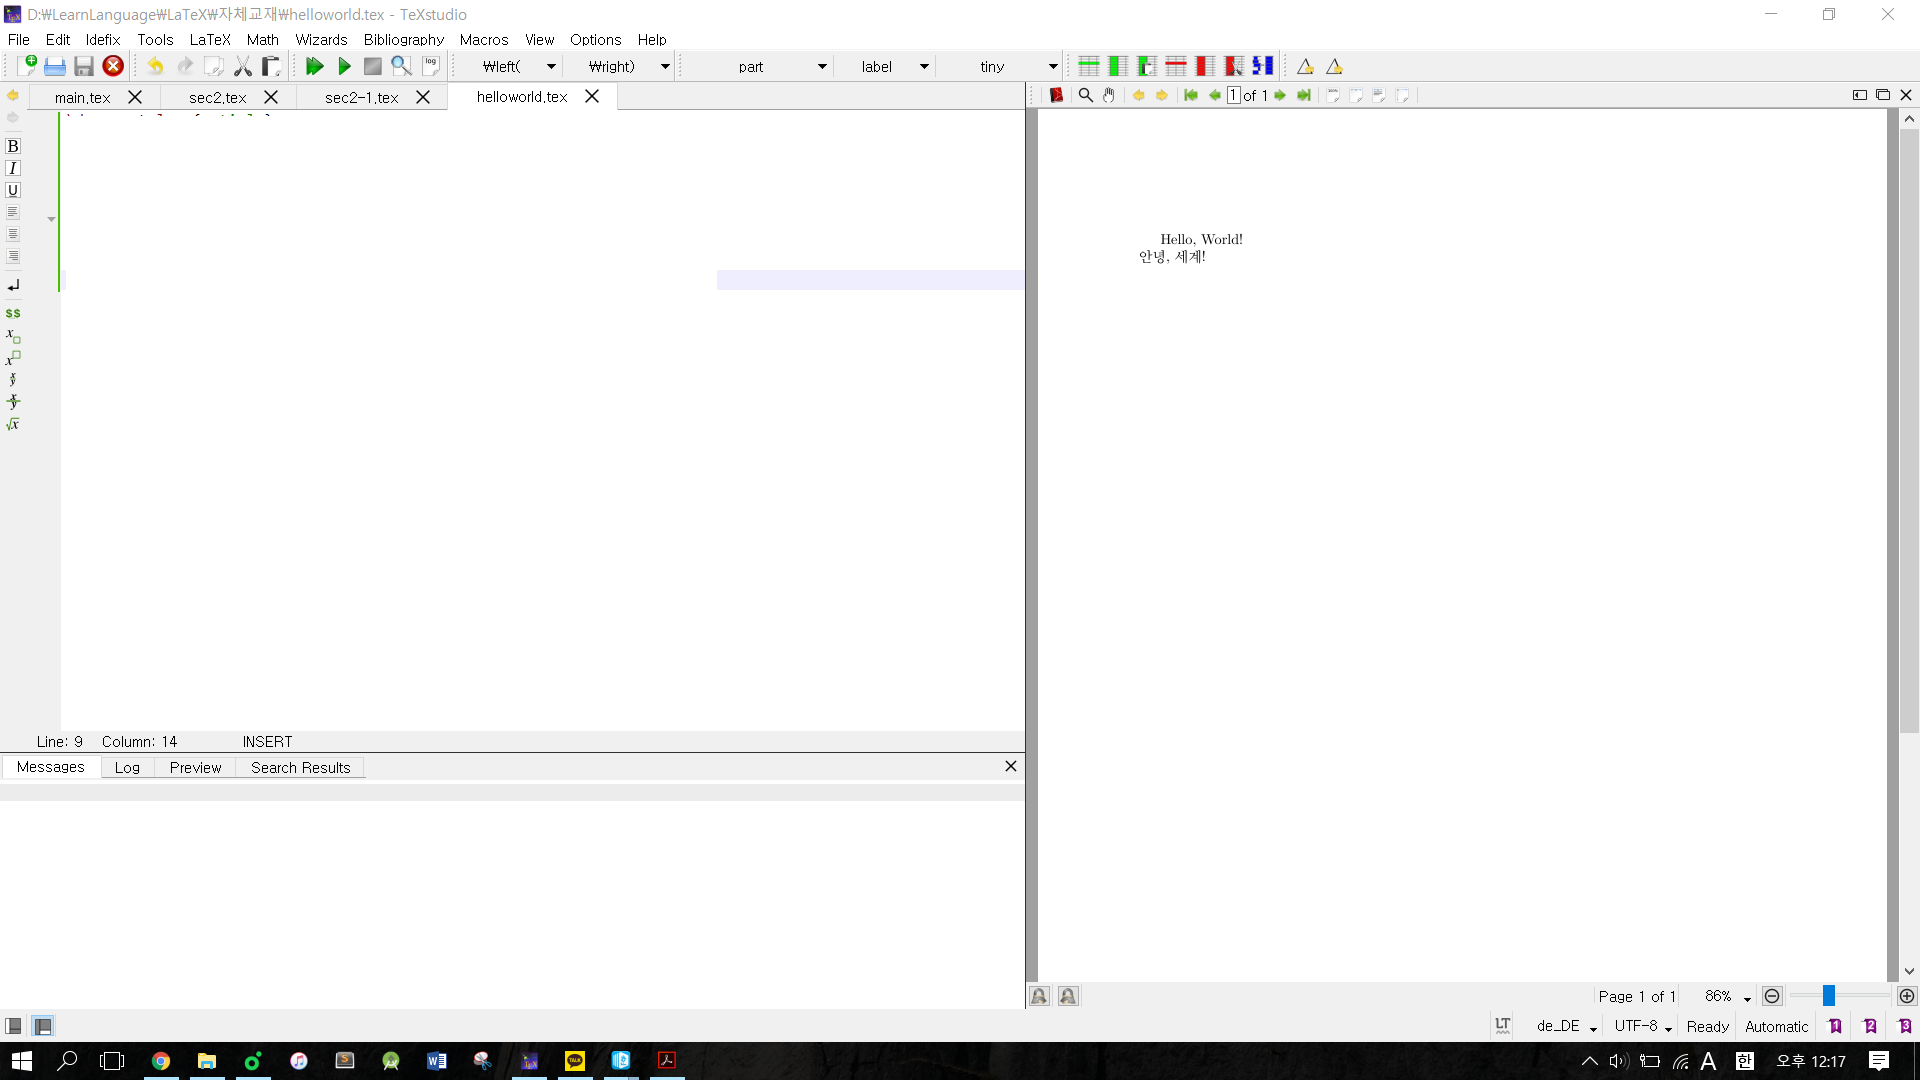
\includegraphics[width=\textwidth]{figures/nhelloworld.png}
	\caption{TeXstudio에서 작업하는 모습\label{fig:nhelloworld}}
\end{figure}

그림 \ref{fig:nhelloworld}처럼 여러분은 에디터를 이용해서 문서를 작성할 수 있어야 합니다. 원하는 문서를 작성하려면 저런 화면에서 계속 타자를 쳐야 하는 겁니다. 그림 기준으로 왼쪽 화면에서 열심히 코딩하듯 입력하면서 오른쪽 화면에 그 결과물을 띄워보고, 또 편집하는 그런 식이죠. 일단 그림 \ref{fig:nhelloworld}에서는 왼쪽 코드를 일부러 가렸습니다. 오른쪽 화면처럼 출력되려면 어떻게 입력해야 할까요?\\
직접 해봐야겠죠? TeXstudio를 실행하고, 파일을 만들어봅시다. 이제부터 차근차근 첫 번째 고비를 해결하는 겁니다.

\paragraph{.tex 파일 생성부터 출력까지}
\begin{enumerate}
	\item TeXstudio를 실행하였다면, 왼쪽 위에 보이는 메뉴들을 봅시다. 새로 문서를 작성하기 위해 파일을 만들어야 하므로, File-New를 클릭하거나 그 바로 아래 아이콘을 클릭합니다. 단축키 Ctrl+N를 이용해도 됩니다.
	\item 이제 뜬 창이 바로 입력 파일을 편집하는 곳입니다. 입력 파일은 미리 저장해둡시다. File-Save를 클릭하거나 아래 디스크 모양 아이콘을 클릭하거나 단축키 Ctrl+S를 이용합니다. 
	\item 입력 파일의 확장명은 tex입니다. (문서파일이름).tex 식으로 파일을 저장합니다.
	\item 이제 입력을 시작하면 됩니다.
          처음이니 깊게 생각하지 마시고 아래의 코드를 따라 쳐 보세요.
    \begin{Verbatim}[frame=single]
\documentclass{article}
\usepackage{kotex}
\usepackage{indentfirst}
\usepackage[left=2.5cm,right=2.5cm,top=3cm,bottom=3cm,a4paper]{geometry}
	
\begin{document}
	Hello, World!\\
	안녕, 세계!
\end{document}
	\end{Verbatim}

	\item 입력이 어느정도 되면 무려 `컴파일'이라는 것을 하게 됩니다. 그래야 문서를 출력할 수 있기 때문입니다.
	\item 컴파일은 역시 위 메뉴에서 찾을 수 있습니다. 초록색 세모 아이콘을 클릭하거나 F6을 누르면 무언가가 돌아가는 모습이 보일 겁니다. `Process exited normally'라는 문구가 아래에 뜨면 성공한겁니다. 에러가 뜰 수도 있습니다.
	\item 컴파일과 동시에 aux, log, out, pdf, synctex.gz, toc 등등 대부분은 알 수 없는 확장자의 파일처음 해보는 들이 생겨납니다. 당황하지 마세요. 잘 진행되고 있는 겁니다.
	\item 컴파일이 성공적으로 끝나면 F7을 눌러봅시다. 오른쪽 화면에 무언가 뜰겁니다. 잠깐만 기다리면 여러분이 입력한 텍스트를 예쁘게 알맞게 출력시키면 어떻게 되는지 뜹니다.
\end{enumerate}

작업 도중 생성된 파일들은 각자 역할이 있고 쓰임이 있지만 일단 꼭 알아야 할 부분만 알아둡시다. 텍스트로 이루어진 tex 파일을 \lt 상에서 실행하여 pdf 파일로 출력물을 얻을 수 있다는 것입니다. 또한 그 상태에서 다시 편집하여 컴파일하면 알아서 변화된 내용대로 파일들이 수정됩니다. TeXstudio를 비롯해 많은 에디터들은 출력결과를 바로바로 확인하면서 편집할 수 있습니다. 이 덕에 \lt 를 WYSIWYG 편집기처럼 사용할 수 있죠.

\paragraph{안녕, 세계!}
가장 기본적인 파일 생성 및 실행, 출력은 위 단계들만 잘 알아두면 됩니다. 계속 문서를 편집하다 보면 자연스럽게 익을 겁니다. 그럼 이제 정말로 어떻게 입력을 해야 문서라는 것이 만들어지는 것인지, 그 내용 부분으로 들어가 봅시다. 앞에 보여드렸던 그림 \ref{fig:nhelloworld}을 다시 생각해 보는 겁니다. 모든 \lt 문서 작성의 기본을, 이 예시를 통해 설명해드리겠습니다.

\lt 은 문서 스타일은 최대한 자동화시켜 알아서 꾸미고, 사용자는 그 내용에 집중할 수 있도록 도와줍니다. 그런 만큼 지금 만드려는 문서가 어떤 종류의 문서인지, 어떤 스타일로 만들어지길 원하는지, 또 어떤 기능을 사용해야 하는지 알려줄 필요가 있습니다. 이 부분을 preamble(서문)이라 합니다. 이제 그림 \ref{fig:helloworld}의 코드를 보면서 이 preamble에 대해 이야기 해 봅시다.

\begin{figure}[h]
	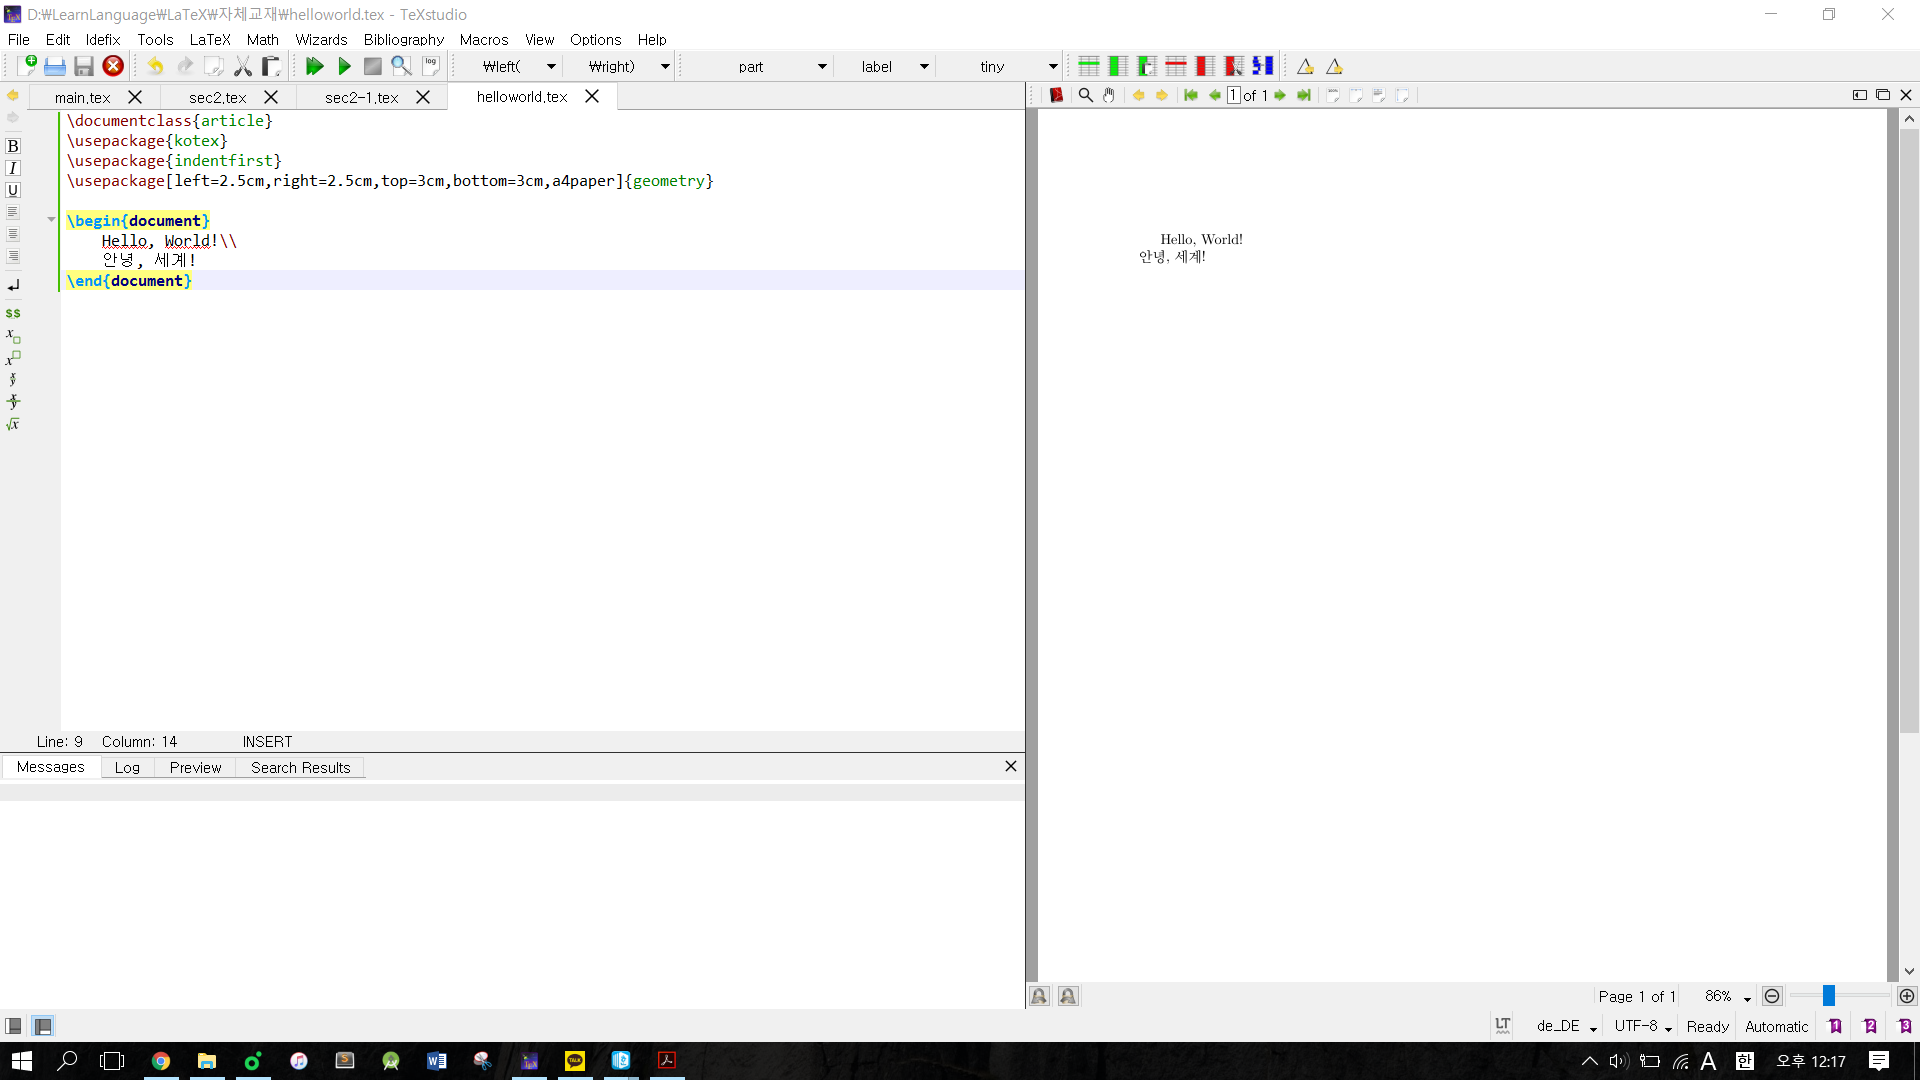
\includegraphics[width=\textwidth]{figures/helloworld.png}
	\caption{기본적인 코드의 모습\label{fig:helloworld}}
\end{figure}

이것이 \lt 문서 작업의 진짜 모습입니다. 코드를 본격적으로 살펴봅시다.

\newpage
\begin{Verbatim}[frame=single]
\documentclass{article}
\usepackage{kotex}
\usepackage{indentfirst}
\usepackage[left=2.5cm,right=2.5cm,top=3cm,bottom=3cm,a4paper]{geometry}
	
\begin{document}
	Hello, World!\\
	안녕, 세계!
\end{document}
\end{Verbatim}

아마 \lt 을 처음 접해보는 분들께는 첫줄부터 무슨 의미인지 이해하기 힘들 겁니다. 천천히 저것들이 무슨 의미인지 봅시다.

\subparagraph{document class}
\label{documentclass}
모든 것의 시작, \verb|\documentclass[option]{class}|부터 이야기할까요? \lt 으로 문서를 작성할 때에는 작성하려는 문서 유형을 처음 선언해주고 시작합니다. 문서 스타일을 자동으로 그 유형에 맞추어 주기 위해서입니다. 이것이 바로 \verb|\documentclass[option]{class}|입니다. class, 즉 문서 유형은 무궁무진합니다. 기본적으로 article부터 letter, beamer까지 9가지 정도의 유형이 있습니다. 각 유형에 대한 설명은 표 \ref{tab:doc cls}을 참고하시기 바랍니다. 물론 저 9가지 class들 외에도 매우 유용하고 좋은 class들이 많이 존재합니다. 이에 대해서는 필요할 때마다 이야기하겠습니다. class를 설정하고 나면 option을 추가로 설정할 수도, 설정하지 않을 수도 있습니다. 설정하지 않는다면 \verb|\documentclass{class}| 식으로 써주시면 됩니다. option에 대한 설명 역시 표 \ref{tab:doc cls opt}를 참고하면 됩니다.

`안녕, 세계!' 예시에서는 article이라는 class를 사용하였습니다. 사실 저정도 내용에서는 다른 class를 사용해도 큰 차이가 없겠지만 각 class마다 그 형태나 사용하는 기능이 다르기 때문에 실제 작성에서는 알맞은 class를 찾아 사용해야 합니다. 예시에서 중요한 점은 단 두 줄 쓰는 데에도 꼭 \verb|\documentclass{}|를 써줘야 한다는 것입니다. 무슨 일이 있어도 첫 줄에 써 주세요!

\subparagraph{begin}
\label{preamble}
문서의 유형을 결정하였다면, 진짜 작성을 시작해야겠죠? 어떤 document class를 선택하든, 그 document의 시작을 선언할 필요가 있습니다. \verb|\begin{document}|를 통해서 말입니다. 이 부분 역시 \lt 작성에서 항상 들어가는 부분입니다. tex 파일에서는 \verb|\documentclass[option]{class}|부터\\
  \verb|\begin{document}|까지를 preamble(서문)이라고 합니다. 여기까지 마친 뒤 여러분이 하려고 했던 이야기들을 적어주시면 되는 겁니다. 또한, 하고 싶은 이야기가 전부 끝났다면, \verb|\end{document}|로 끝마쳐야 합니다. 이것이 모든 문서의 기본입니다.그림 \ref{fig:helloworld}를 보시면 잘 나와 있듯이, 저렇게 문서의 모든 내용을 감싸주고 있다고 생각하시면 됩니다. 참고로, \verb|\begin{}, \end{}| 구문은 굉장히 많은 용도로 쓰이기 때문에 잘 알아두셔야 합니다.

  \subparagraph{package}
  \label{sec2-package}
혹시 기본적인 것만으로는 표현할 수 없는 무언가를 표현해야 한다면, package를 찾게 될 겁니다. \verb|\documentclass[option]{class}|와 \verb|\begin{document}| 사이에는 해당 문서에서 특정 package를 사용할 수 있도록 선언해주는 \verb|\usepackage[option]{package}|가 들어갈 수 있습니다. 마치 Python에서 사용할 모듈을 import하듯이 사용해야 하는, 사용하려는 package를 미리 불러오는 거죠. Python에서 모듈이 무궁무진하듯, package 역시 많은 사람들이 개발하고 있기 때문에 굉장히 다양하고, 얼마든지 필요한 package를 찾거나 직접 만들어서 추가할 수 있습니다. 그림 \ref{fig:helloworld}의 '안녕, 세계!'라는 한글 역시 kotex라는 package를 추가하였기 때문에 사용할 수 있는 겁니다. 자주 쓰이는, 주요 package들에 대해서는 앞으로 차차 소개해 드릴 겁니다.

위 세가지를 잘 기억해두고, 잘 써먹으면 \lt 문서의 기본이 완성된 것입니다. 이제 하고 싶은 이야기를 입력해 주시면 됩니다.

\paragraph{문제가 생기셨나요?}
\label{sec2:problem}
컴퓨터에 익숙하지 않으신 분들은 시작부터 문제가 생기기도 합니다.
하지만 겁먹으실 필요는 없습니다.
지금부터 문제의 소지가 있을 만한 부분을 하나씩 짚어보도록 하죠.
\begin{itemize}
	\item \TeX \emph{live 설치 창}에서 문제가 생기셨으면 여기를 봐 주세요.
	한글 텍 사용자 그룹에서 권하는 대로 폴더 변경이 안 되나요?
	사실 굳이 폴더를 변경하실 필요는 없습니다만, 오류가 생기는 이유는 \TeX Live 설치 프로그램이 새로운 폴더를 자동으로 생성해주지 않기 때문입니다.
	수동으로 원하는 폴더를 생성하고 다시 시도해 보세요.
	
	\item \emph{커맨드창}이라고 불리는 것들은 명령 프롬프트입니다.
	Windows 검색창에서 검색하셔서 실행하시면 됩니다.
	참고로 커맨드창에서 tlmgr 명령을 하실 때는 커맨드창을 관리자 권한으로 실행시키셔야 합니다.
	오른쪽 클릭하시면 하실 수 있습니다.
	
	\item TeXStudio가 한글 입력이 원활하지 않을 수 있습니다.
	가끔 그런 경우가 있더라고요.
	이건 그냥 그 프로그램상의 오류니까 굳이 깊게 생각하지 마시고 다른 에디터를 사용하세요.
	에디터는 다양합니다.\footnote{\url{http://tex.stackexchange.com/questions/339/latex-editors-ides}}
	자신에게 맞는 에디터를 골라보세요.
	
	\item \lt 에만 해당되는 사항은 아니지만, 항상 오류가 나면 가장 먼저 의심해 보아야 할 것은 \emph{한글}입니다.
	안타까운 이야기지만 세계적으로 보았을 때 한글을 잘 처리할 수 있는 소프트웨어가 그다지 많지 않습니다.
	어떤 프로그램이 실행되는 경로상에 한글과 같은 non-ASCII code가 포함되어 있으면 오류가 나는 경우가 상당히 많죠.
	그런 의미에서 폴더 이름은 되도록 영어로 하는 것이 좋습니다. 꼭 \lt 만을 위해서가 아니더라도요.
	같은 맥락에서 Windows 사용자 이름이 한글로 되어 있으면 프로그램 설치에 문제가 생길 수 있습니다.
	\lt 나 TeXStudio의 경우에는 어떤지 확실하게는 말씀드리기 어렵지만 문제가 생기신다면 의심하실 필요는 있습니다.
	이건 윈도우를 초기화하지 않는 이상 바꾸기 상당히 까다로우니 주의해 주세요.
	개인적으로는 초기화를 하더라도 바꾸는 것을 권장합니다.
	다른 수많은 프로그램들을 위해서라도요.
	
	\item 아 그리고 참고로 알아두셨으면 하는 게 있네요.
	아마 여러분이 pdf 파일을 보는 데 Adobe Acrobat Reader를 쓰시는 경우가 많으실텐데, 이 프로그램은 완성된 문서의 결과를 보는 데만 쓰셨으면 합니다.
	Acrobat Reader는 자신이 읽고 있는 pdf 파일을 잠급니다.
	다시 말해 Acrobat Reader로 pdf 파일을 켜 놓으셨으면 그 파일은 \emph{컴파일이 되지 않을 겁니다}.
	\lt 전용 에디터들의 내장 뷰어나, SumatraPDF와 같은 프로그램은 특정 파일을 읽는 동안에도 그 파일의 수정을 허용하고, 뷰어를 껐다 켜지 않더라도 새로고침할 수 있지만, Acrobat은 그렇지 않습니다.
	꼭 Acrobat만 그런 건 아니겠지만요.
	어쨌든 pdf 뷰어를 켜놓고 컴파일이 되지 않는 경우 자신이 사용하는 pdf 뷰어의 특성일지 모른다는 것도 염두에 두셔야 합니다.
	
      \end{itemize}
      여기에 없는 문제들은 친구에게 물어보거나, 구글에 검색해 보세요. 아마 여러분과 같은 어려움을 겪고 있는 사람들이 상당히 많을 겁니다.

%%% Local Variables:
%%% mode: latex
%%% TeX-master: "main"
%%% End:
